\chapter{Materials and Methods} \label{material_methods}

\section{Research area} \label{research_area}
The Canton of Zug was chosen by the author who was raised in the town Cham as the area of interest since local knowledge was seen as an important asset and due to the manageable spatial extent. The specific areas for which social media data (SMD) was acquired are visible in the map of figure \ref{fig:research_area}. The turquoise area resembles the political border of the Canton of Zug for which SMD for the social media platforms (SMP) Flickr and Foursquare were collected. The purple area is included in the above mentioned perimeter and consists of three major areas. In the North lies the 'Lorzenebene' (plane of the river Lorze). This area is of special interest to the cantonal authorities due to its local recreation value. An overall concept named 'Leitbild Lorzenebene'  \parencite{BaudirektiondesKantonsZug2012} has been created for that area which outlines the future development goals also in regard to potential nature-based recreation services. The second area resembles the jurisdiction of the city of Zug which partly encompasses the 'Lorzenebene'. This area is characterised by its internal urban gradient which increases towards the city centre as well as the long reaching lake side. The last area furthest South consists of the three mountains 'Zuger-, Walchwiler-, Rossberg' which are likewise part of an development concept \parencite{Berchtold2011} of the Canton of Zug due to their among others sport and recreation value. \\
There is no perimeter concordance due to varying constraints in the data acquisition between the different SMPs which will be illustrated in the following subsection.

\begin{figure}[h]
   \centering
   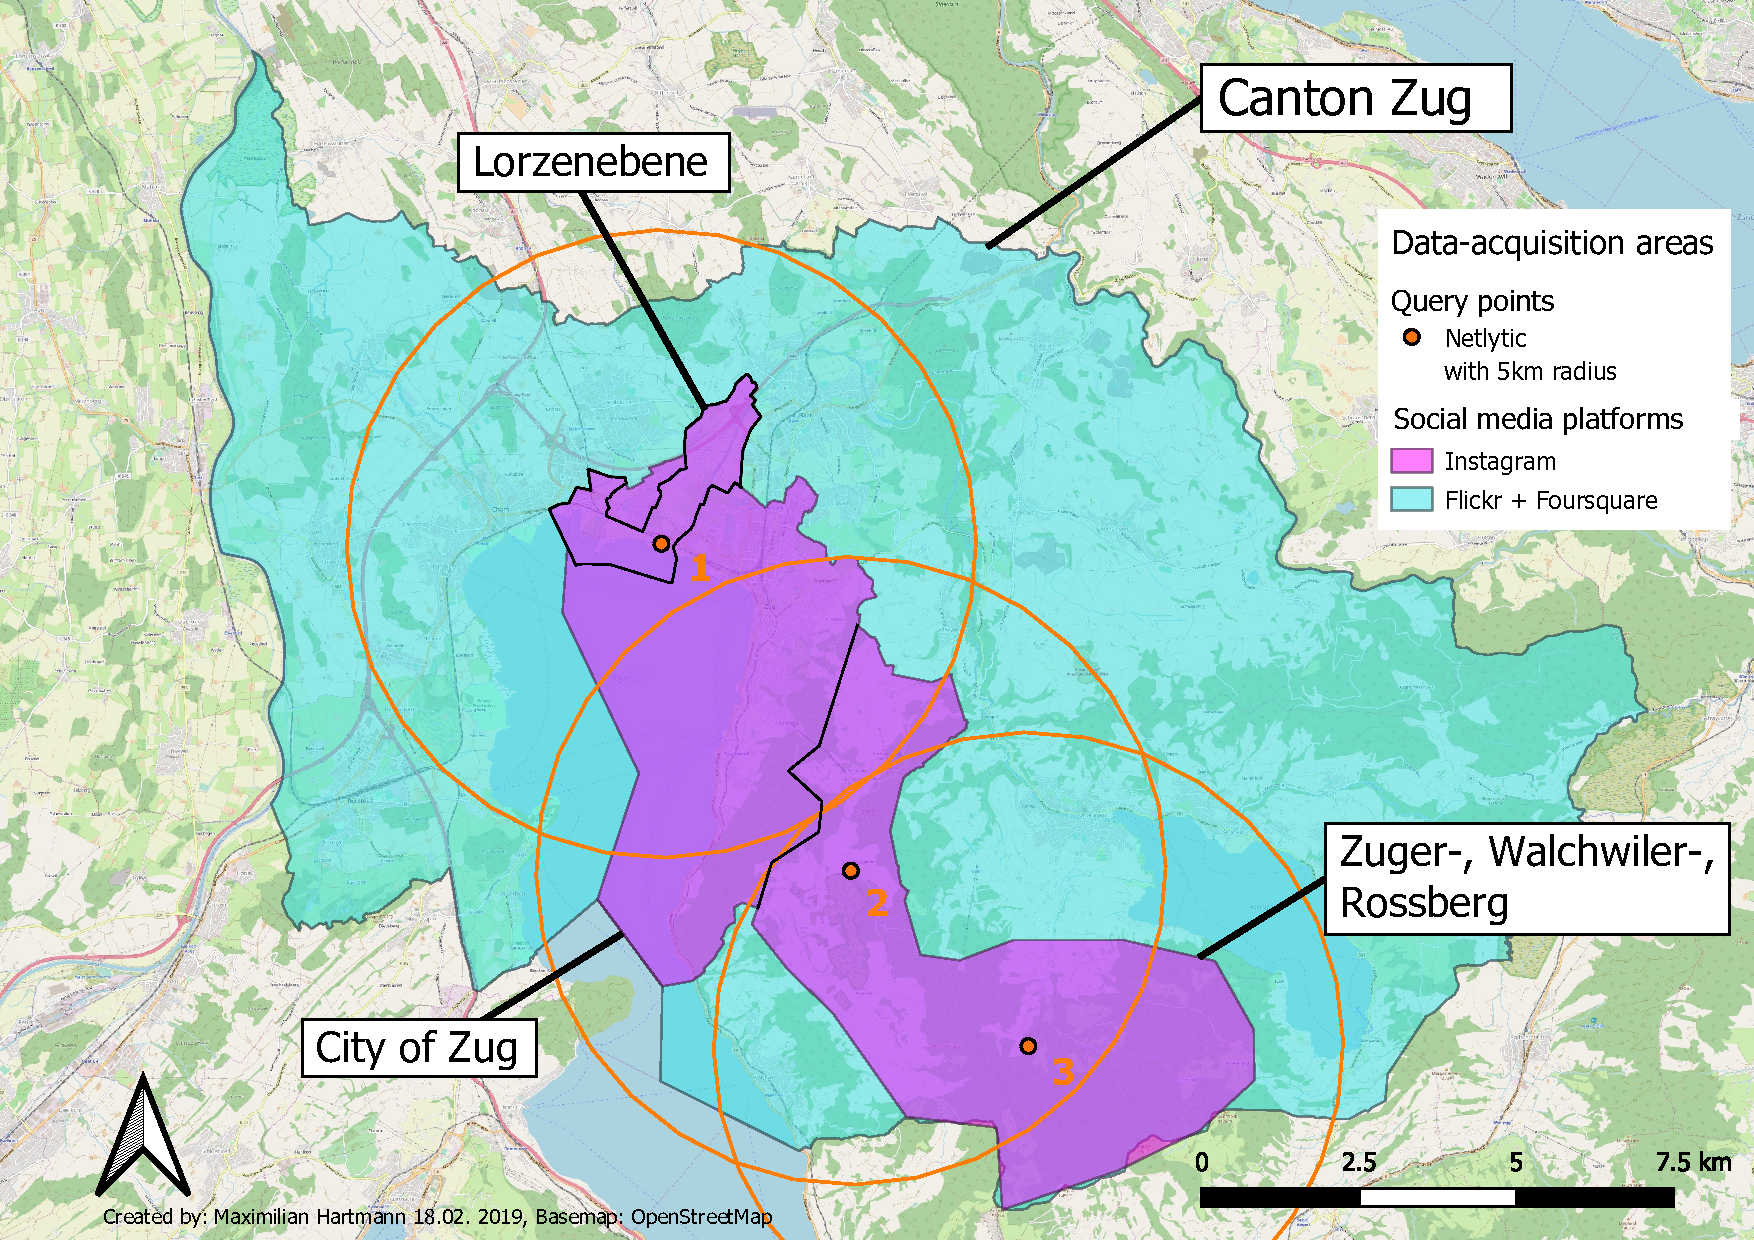
\includegraphics[width=0.75\textwidth]{img/overview_research_area_w_Lorzenebene}
   \caption{Overview of the data acquisition perimeters}
   \label{fig:research_area}
\end{figure}


\section{Data acquisition and composition} \label{data_acquisition}
The following subsections will elaborate on the data-acquisition process and the data-composition of the three SMPs used in this thesis. 

\subsection{Instagram} \label{instagram}
Instagram\footnote{https://www.instagram.com/} is a SMP which supports the sharing of georeferenced image and video content. The platform is mostly financed by web-advertisement and belongs to Facebook\footnote{https://www.facebook.com/}. Instagram held roughly 2'529'000 users in Switzerland on January 2019 which accounted for 29.4\% of its population. People aged 25 to 34 were the largest user group (780'000). The gender distribution was at 49.4\% women and 50.6\% men\footnote{https://napoleoncat.com/stats/instagram-users-in-switzerland/2019/02, accessed: 30.03.2019}. This popularity was the determining factor for using Instagram data in this thesis.\\

\subsubsection*{Query} \label{netlytic}
Licensed Instagram data of the research area visible in figure \ref{fig:research_area} has been collected via the cloud-based text and social media analyser Netlytic\footnote{https://netlytic.org/} \parencite{Gruzd2016}. Netlytic allows for hashtag (\# + keyword) as well as location driven queries. Former allows to search for Instagram media objects by providing decisive keywords which are preceded by a '\#'. The latter was used in the scope of this thesis which allows to collect Instagram media objects of public accounts in a 5km radius around a given coordinate. These Netlytic query points with their given perimeter are also visible in figure \ref{fig:research_area}. The exact latitude / longitude pairs are the following:\\
\begin{enumerate}
  \item 47.177068, 8.494803
  \item 47.129913, 8.533604
  \item 47.104457, 8.570291
\end{enumerate}

\subsubsection*{Time-span} \label{Instagram_timespan}
Data collection has been continuously performed on all three coordinates from the 30.09.2018 till the 11.12.2018. Due to the retirement of the Instagram Application Program Interface (API) on the 11.12.2018 this period could not be extended\footnote{https://www.instagram.com/developer/, accessed: 29.03.2019}.

\subsubsection*{Data} \label{Instagram_data}
The data-collection accounted for 28'246 raw Instagram media objects. After the dominant authors and bulk-upload data-processing steps referenced further down (see section \ref{data_processing}) 11'777 remained.
The data provided by Netlytic came in the Comma Separated Values (CSV) format. Every media object was provided with the following information entities with the appropriate PostgreSQL data type in square brackets:
\begin{itemize}[label={}]
    \item \textbf{id:} Unique media object identifier. \big[varchar(30)\big] if the media object contains location information, \big[numeric(20)\big] if not.
    \item \textbf{latitude and longitude
    :} Coordinate information in the WGS84 reference system of a specific Instagram location \big[double precision\big]
    \item \textbf{link:} URL to the actual media object on \texttt{https://www.Instagram.com/} \big[text\big]
    \item \textbf{media-link:} URL directing solely to the image content \big[text\big]
    \item \textbf{publication date:} Date and time when the media object was uploaded in the data-format \texttt{YYYY-MM-DD HH:MM:SS} \big[timestamp\big]
    \item \textbf{author:} The Instagram username of the media object author \big[text\big]
    \item \textbf{title:} User generated media object title \big[text\big]
    \item \textbf{description:} User generated media object description \big[text\big ]
    \item \textbf{like-count:} Amount of likes the media object received on the SMP Instagram \big[bigint\big]
\end{itemize}

\subsubsection*{Location tag} \label{instagram_location_tag}
The provided location information or tag consists of the above mentioned coordinates of an Instagram location. Instagram locations are points of interest which can be user-generated and must not represent the actual precise coordinates where the media object was created. This has been implemented by Facebook as a further step to preserve the Instagram users anonymity by mitigating the divulging of sensitive location data. This implies that media objects that do not originate from the same location can still be 'snapped' to the same Instagram location and therefore show the same coordinate pair in the meta-data \parencite{Instagram}.
It has been shown that roughly 85\% of Instagram media objects lack a location tag and most users only use them on vacation or when being abroad \parencite{Flatow2015}.
Additional location related information (address) was gathered for all the media objects via the official Instagram API. More information can be found in section \ref{geolocation_via_instagramapi}.



\subsection{Flickr} \label{flickr}
Flickr\footnote{https://www.flickr.com/} is a photo sharing website that allows users to upload georeferenced images similar to Instagram. The corresponding free of charge Flickr API gives

\renewcommand{\thefootnote}{\alph{footnote}}

access to the entire database of Flickr media objects since the launch of the platform in the year 2004. The popularity of Flickr according to the 'Alexa Global Rank' lies at 349\footnote{https://www.alexa.com/siteinfo/flickr.com, accessed: 29.03.2019} which is significantly lower than to the one of Instagram which lies at 16\footnote{https://www.alexa.com/siteinfo/instagram.com, accessed: 29.03.2019}. \textcite{Tenkanen2017} states that in the period between 2004 and 2017 over six billion images were uploaded by 71 million Flickr users of which roughly 197 million images or 3.3\% were geo-referenced. 

\renewcommand{\thefootnote}{\arabic{footnote}}

Flickr still plays an important role as data foundation for scientific studies due to the simple and unbounded data-access. 
\subsubsection*{Query} \label{flickr_query}
The entire Flickr database was queried via the publicly accessible official Flickr API. Media objects with a georeference-accuracy level of 12 or higher (maximum of 16) were of interest which resolves to city level up to street level. Multiple queries with variable bounding boxes were performed which together cover the entire perimeter of the legal boundaries of the Canton of Zug. Each bounding box was defined by two coordinate pairs, describing the bottom left and top right corner of a rectangle. This process of subdividing the area was necessary due to a maximum return threshold of 4'000 media objects per request. Therefore, to ensure the acquisition of the entire available dataset each bounding box had to hold less than 4'000 media objects.

\subsubsection*{Time-span} \label{flickr_timespan}
All Flickr API requests described above were queried for the time-spawn 2004 (launch of the SMP Flickr) until the 23rd of November 2018.

\subsubsection*{Data} \label{flickr_data}
The data that was returned by the Flickr API was in the JavaScript Object Notation (JSON) format. The following information has been extracted for every Flickr media object with the appropriate PostgreSQL data types in square brackets:\\

\begin{itemize}[label={}]
    \item \textbf{id:} Unique media object identifier \big[bigint\big]
    \item \textbf{latitude and longitude:} Coordinate information in the WGS84 reference system \big[double precision\big]
    \item \textbf{link:} URL in the form \texttt{https://www.flickr.com/photos/[author]/[ID]/} to the actual media object \big[text\big]
    \item \textbf{date taken:} Time-stamp from the image meta-data stating when it was taken \big[timestamp\big]
    \item \textbf{publication date:} Time-stamp when the media object was uploaded to Flickr with the data-format \texttt{MM/DD/YYYY HH:MM:SS} \big[time-stamp\big]
    \item \textbf{author:} The Flickr username of the media object author \big[text\big]
    \item \textbf{author id:} Unique author identifier \big[text\big] 
    \item \textbf{author origin:} User given geographical information regarding the authors origin \big[text\big]
    \item \textbf{title:} User generated media object title \big[text\big]
    \item \textbf{description:} User generated media object description \big[text\big]
    \item \textbf{tags\footnote{https://help.flickr.com/en\_us/tag-keywords-in-flickr-BJUJpQoyX, accessed: 29.03.2019}:} Keywords similar to Instagram hashtags that describe the media object but which are extracted by an image recognition algorithm similar to Google Cloud Vision. (therefore already includes smart image labels) \big[text\big]
    \item \textbf{views:} Amount of media object calls \big[bigint\big]
    \item \textbf{favourites:} Amount of approves similar to 'likes' on Instagram a media object received by other Flickr users \big[bigint\big]
\end{itemize}

\subsubsection*{Location tag} \label{flickr_location_tag}
Flickr provides unlike Instagram location information or tags that represent the actual geographical position where the provided image was taken. This geotag is extracted from the meta-data of the image and can come in different accuracies ranging from 0 (global scale) to 16 (street level) dependant on the users preference or the GPS signal strength. \\
Additional location related information (address and location type) was gathered for all the Flickr media objects via the Google Geocoding API. More information can be found in section \ref{geocoding_api}

\subsection{Foursquare} \label{foursquare}
Foursquare\footnote{https://de.foursquare.com/} is a platform which enables users to rate and share their visits and experiences to certain establishments (referred to as venues). This stored infrastructure which is categorised into different sectors such as \textit{Travel \& Transport}, \textit{Arts \& Entertainment} but also \textit{Outdoors \& Recreation} can be accessed via the official Foursquare API.

\subsubsection*{Query} \label{foursquare_query}
The following two API endpoints which return different information were used for this thesis.
\paragraph*{Venue search (regular endpoint)} \label{foursquare_endpoint1}
The first step of the data-acquisition involved a spatial search for venue ids of the category \textit{Outdoors \& Recreation} that lie within the boundaries of the Canton of Zug. This request was done with the regular venue search API endpoint. There is a limitation to the maximum number of results per request in place similar to the bounding box request of Flickr. Therefore, a spatial subdivision of the research areas was again used to query all the available venues so that each individual request returned less than 50 results.
\paragraph*{Acquiring venue details (premium endpoint)} \label{foursquare_endpoint2}
To obtain more specific information about each venue a second (premium) Foursquare API endpoint was used. This venue endpoint allows regular (non-paying) users 50 requests per day which spread the data acquisition over 9 days for a total of 405 available venues. The results included insight on a more concrete subcategory description, the formatted venue address, the users rating as well as if the venue was verified or not.

\subsubsection*{Data} \label{fq_data}
The data returned by the Foursquare API with the above mentioned endpoints was in the JSON format - the same as the Flickr data.
The following excerpt of the returned venue meta-data was further used in this thesis with the appropriate PostgreSQL data types in square brackets: \\
\begin{itemize}[label={}]
    \item \textbf{venue id:} Unique venue identifier \big[text\big]
    \item \textbf{venue name:} Locally used name to address the venue \big[text\big]
    \item \textbf{latitude and longitude:} Coordinate information in the WGS84 reference system \big[double precision\big]
    \item \textbf{country name:} Name of the country the venue is located in - used as additional data-verification \big[text\big]
    \item \textbf{rating:} Foursquare users generated venue rating \big[real\big]
    \item \textbf{category id:} Unique venue category identifier \big[text\big]
    \item \textbf{category name:} Venue category name \big[text\big]
    \item \textbf{verified:} Takes the values True or False. States if the venue data is verified by Foursquare \big[boolean\big]
\end{itemize}

Additional location related information (address and location type) was gathered for all the Foursquare venues via the Google Geocoding API. More information can be found in section \ref{geocoding_api}.

\subsubsection*{Data verification} \label{foursquare_data_verification}
The data verification on Foursquare is not an automated process. It is done by manual supervision of Foursquare personnel. A business can claim their venue which will initiate the Foursquare verification process. This processing is linked to a fee of roughly 20 US-Dollars\footnote{https://support.foursquare.com/hc/en-us/articles/201063930-How-to-claim-your-listing-s-, accessed: 29.03.2019} for venues outside of the United States of America. \\
Of all 405 venues located inside the Canton of Zug, 13 (3.2\%) are verified according to the data provided by the Foursquare API. The remaining non-verified venues of the categories: scenic outlook, playground, athletics \& sport, farm, (nudist) beach, lake, trail, golf course, mountain, campground, bathing area, outdoors \& recreation, harbour, recreation centre, dog run, forest, pedestrian plaza, waterfront, basketball court, river, bike trail and skate park were validated by the author to its best knowledge. The final Foursquare dataset encompassed 378 venues.

\section{Database setup} \label{database_setup}
A PostgreSQL\footnote{https://www.postgresql.org/} database was used as a centralised storage hub for the Flickr, Instagram and Foursquare data. The advantage of a database compared to reading and storing data in TXT- or CSV-files is the computational efficient data-retrieval and data-manipulation through SQL queries. SQL is a standalone language for relational database management systems (RDBMS) which allows among others smart table joins and advanced filtering as stated in the official PostgreSQL Documentation\footnote{https://www.postgresql.org/files/documentation/pdf/11/postgresql-11-A4.pdf, accessed: 29.03.2019}.\\
Additionally, a Graphical User Interface (GUI) named pgAdmin4\footnote{https://www.pgadmin.org/} - which is build on top of PostgreSQL - was used for the manually performed training's data verification process that is described in section \ref{precision_unseen_data}.\\
The following tables were created for housing the used data in this format:\\ \texttt{[object-type]\_[data-origin]\_[SMP]} \\
\newline

Media object tables:

\begin{itemize}
    \item \texttt{media\_objects\_cantonzug\_flickr}
    \item \texttt{media\_objects\_unionzug\_instagram}
    \item \texttt{media\_objects\_trainingdata\_instagram}
    \item \texttt{media\_objects\_cantonzug\_foursquare}
\end{itemize}

Location tables:

\begin{itemize}
    \item \texttt{locations\_cantonzug\_flickr}
    \item \texttt{locations\_unionzug\_instagram}
\end{itemize}

In more detail the media object tables store all data related to an object retrieved from one of the three SMP as stated in the subsections above. Furthermore, the outputs from the data- and text-processing steps (see section \ref{data_processing}) are stored in the database. The exact structure and table specific content of the PostgreSQL database is visible in figure \ref{fig:database}. The Instagram and Flickr media object tables are linked via a primary key to the corresponding locations table where unique media object location information is separately stored to reduce redundancy. This information exceeds the basic coordinates provided by the Flickr API and the stand-alone user generated locations provided by Netlytic (Instagram). Additional geographic information was acquired via the Googles Geocoding API and the Instagram API respectively (see section \ref{add_location_data}). Time-stamps were normalised across all SMP to the \texttt{YYYY-MM-DD HH-MM-SS} format.

\begin{figure}[h]
   \centering
   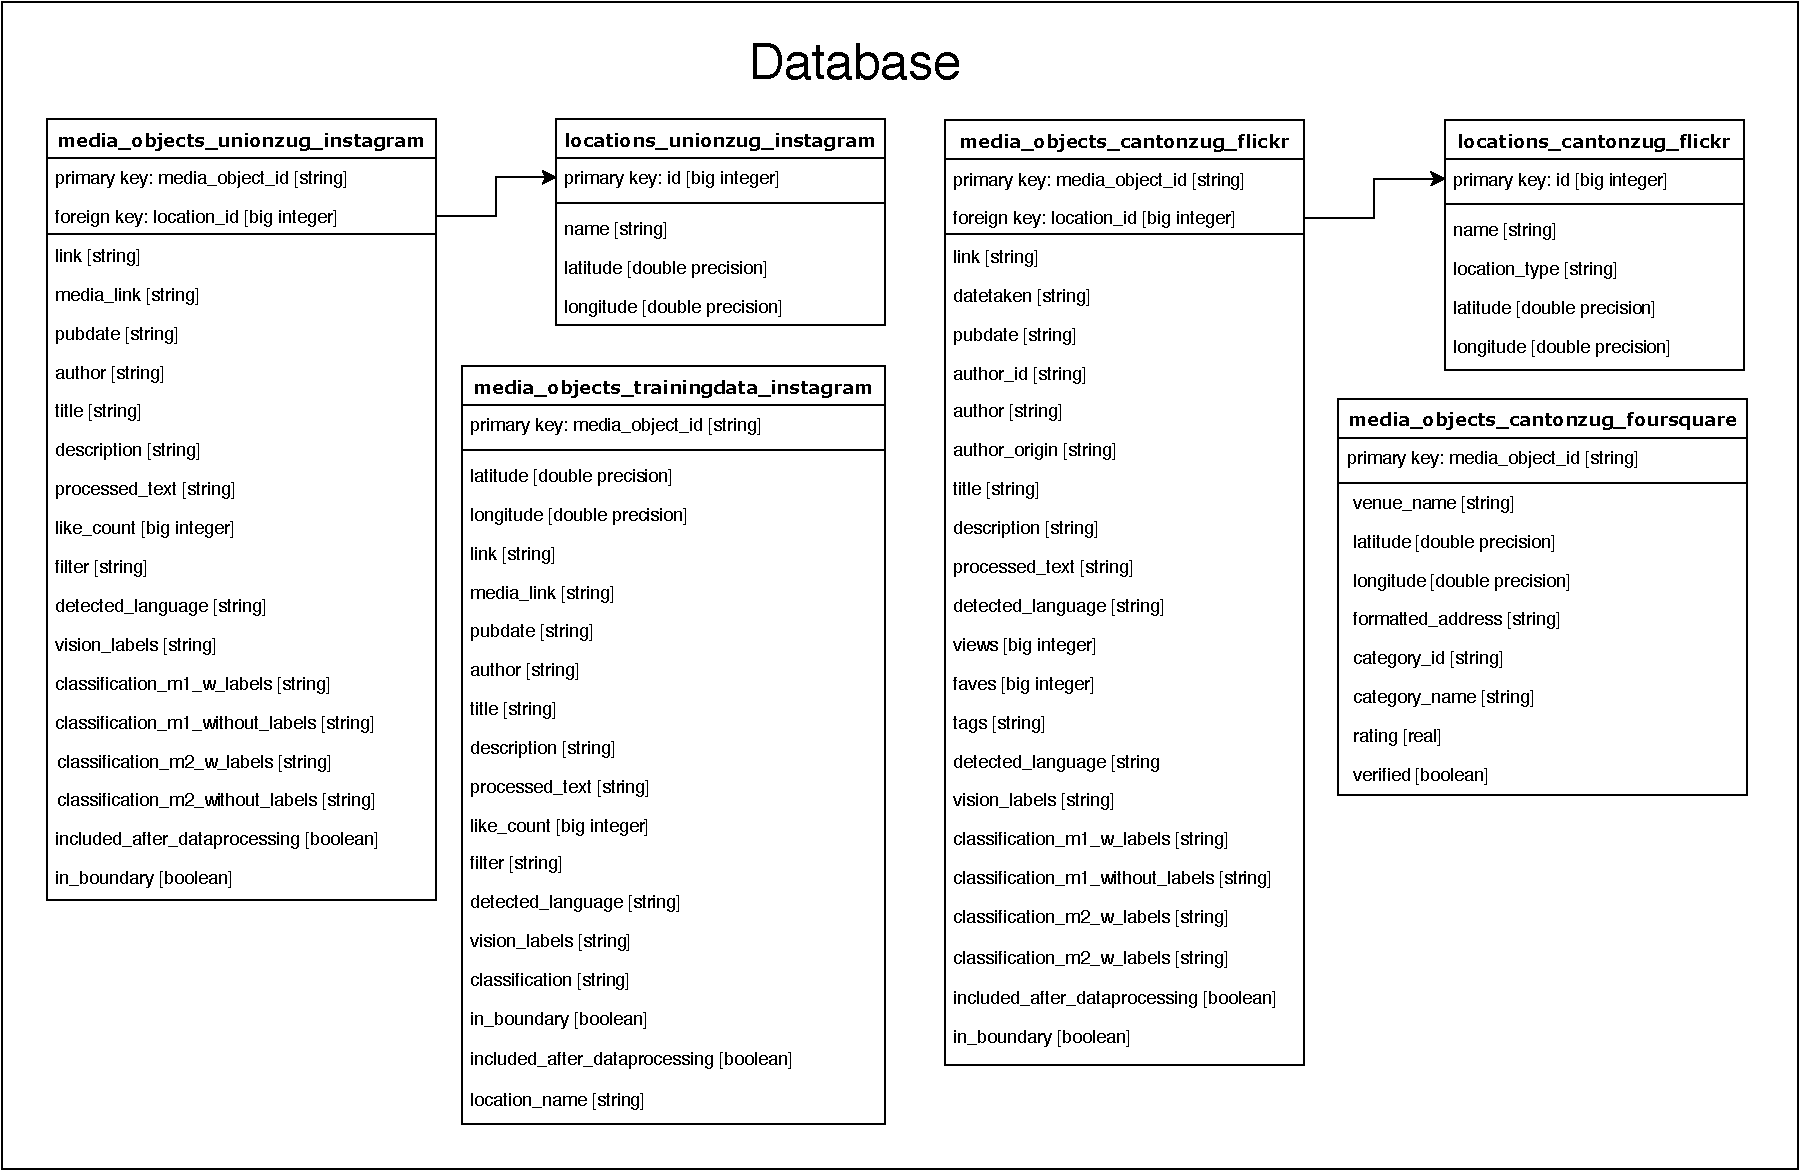
\includegraphics[width=0.75\textwidth]{img/fusion_db_overview}
   \caption{Visualisation of the database, its associated tables and columns. \\ Created with https://www.draw.io/}
   \label{fig:database}
\end{figure}

\texttt{Remark:} The entire populated database in its final form can be found on the enclosed CD.

\section{Data-processing} \label{data_processing}
The following processes cover the entire workflow of data manipulation on the database in the order they were performed.
\subsection{Merging of Instagram files} \label{netlytic_files_merge}
In total, three different partly spatially overlapping Netlytic queries were run to acquire the needed Instagram data. All of them returned one CSV-file. These files were merged for simplicity reasons and media object duplicates were simultaneously removed in the process. This entire step was not needed for the Flickr-data since merging and duplicates were already handled during the data-mining process.

\subsection{Acquisition of additional location information} \label{add_location_data}
Auxiliary, more detailed location information regarding the spatial origin of the media objects in the database were acquired. The following two subsections will elaborate on this process for the different data sources Instagram and Flickr.

\subsubsection*{Via the Instagram API} \label{geolocation_via_instagramapi}
The Instagram data that was provided by Netlytic was enhanced by using the \\ \texttt{GET/locations/location-id} endpoint of the official Instagram API. Newly acquired information encompassed the Instagram location-name.

\subsubsection*{Via the Google Geocoding API} \label{geocoding_api}
Each coordinate of every Flickr media object was run through the Google Geocoding API. Detailed information regarding the media object's address and location type was returned. The location type attribute is evidence of the API's accuracy. Everything besides \small{\textit{ROOFTOP}} returns an address that is close but not exactly at the given coordinate and therefore represents a spatial approximation. The API has been called by modifying the following HTTPS-request:\\
\texttt{\footnotesize{https://maps.googleapis.com/maps/api/geocode/json?latlng=[latitude,longitude]\&key=[API\_KEY]}}

\subsection{Populating the database} \label{populate_db}
The merged Instagram CSV-files and the Flickr CSV-files which were extended by the additional location information described in the subsections above were used to populate the initial PostgreSQL database. This process was entirely performed with the script provided in Appendix \ref{python_code} and the needed \textit{psycopg 2} Python library that functions as linkage to the database.

\subsection{In boundary condition check} \label{in_boundary}
Additional unwanted data beyond the actual research area boundaries was included due to the circular (Netlytic; see figure \ref{research_area}) or rectangular (Flickr API) shape of the spatial query perimeters. As consequence each acquired media object was checked to be inside the actual perimeter boundary. This process was accomplished with an open source Geographical Information System (GIS) named QGIS. The point data of all media objects was clipped to the appropriate research area and exported to a new CSV-file. This CSV-file was read by the Python script which updated the \texttt{in\_boundary} column to \textit{True} for the provided media objects.

\subsection{Addressing sources of data-bias} \label{sources_data_bias}
This part of the data-processing is a filtering step as seen in step 1 of figure \ref{fig:ml_visualisation} to eliminate media objects which would distort the \textbf{general} perception of the research question at hand: Where are people performing NBRAs?

\subsubsection*{Dominant authors} \label{bias_dominant_authors}
Authors (people who contribute to a given social media platform by uploading media objects) who are above a certain threshold regarding their total number of uploaded media objects in the research area during the data-acquisition period are marked in the database table column \texttt{included\_after\_dataprocessing} as \texttt{False} and are thereby excluded from further analysis. There is a need to address dominant authors because drawn conclusions will be otherwise based on a small number of users that contributed a large share to the entire data-set.\\
\newline
\textbf{How was this threshold defined?}\\
\newline
Two possibilities were considered:
\begin{enumerate}
  \item A static top percentage of authors will be excluded
  \item A variable dataset-specific amount of the most contributing authors will be excluded
\end{enumerate}

At first a static top 0.5\% threshold was implemented across all data-sets. Later in the development of the thesis possibility 2 was implemented. A 'posts per author' distribution graph (e.g. see figure \ref{img:dominant_users_flickr}) is simultaneously created as soon as data is read into the database. The number of desired top authors which should be included in the graph can be manually adjusted. This enabled a data specific dynamic adaption of the threshold according to a visual evaluation of the graph and the underlying data-set. 

\subsubsection*{Bulk uploads} \label{bias_bulk_uploads}
In the context of this thesis bulk uploads describe a certain amount of simultaneously or during a short period of time uploaded media objects to the same social media platform by a single author. In an early stage of the project a static bulk upload threshold - similarly to the dominant author threshold - was chosen. Later, a dynamic solution which makes adaptive data handling possible was implemented. A graph which visualises the amount of effected media objects by different bulk upload thresholds (2-10) is displayed to the user (see figure \ref{img:bulk_uploads_flickr}). According to the graph a suitable threshold can be inputted and applied to the given dataset. The time period in which the exceeding of the threshold was considered a bulk upload was set to one hour. 
All as bulk upload marked media objects will be excluded from further analysis by setting the \texttt{included\_after\_dataprocessing} column to \textit{False} (if they were not already excluded in the 'dominant user' step).

\subsection{Text-processing} \label{text_processing}
Text processing is required to turn noisy user-generated character input (text) into normalised word-tokens which are comparable between media objects. These tokens are a prerequisite for the following machine learning (ML) text-classification approach. The text-processing encompasses the following steps in corresponding order which have been visualised under step 3 in figure \ref{fig:ml_visualisation}: Firstly, iterating over all media objects which lie inside the research area boundary and are included after the data-processing while acquiring the corresponding text-data from the database.

\subsubsection*{Language detection} \label{language_detection}
The language detection serves the purpose of optimally adjusting the parameters for the later performed core text-processing step. By identifying the language, a matching word lists can be chosen to check the spelling, remove meaningless stop words as well as stem words to its roots (see \ref{core_text_processing}).\\
To accomplish a text string which consists of the media object's title is parsed to the function. Firstly, basic text-processing is necessary to ensure a reliable prediction which consists of splitting the text-string at white spaces. Next, any sort of URI (universal resource identifier), HTML, common geographic references (such as the city of Zug) and character/number combination-patterns are removed with the help of regular expression matching. Lastly, all characters are turned lowercase. The resulting word-tokens are only further considered if they have a minimum length of three characters. This minimum length was chosen according to conducted tests to avoid short character-artefacts that can occur during the described process.\\
In a following step each created word-token is run against five different word lists of the English, German, Swiss German, French and Italian language.
The English word list was acquired via the \textit{natural language toolkit} (NLTK) Python library. The mentioned list encompasses over 236'000 of the most common words of the English language.
The German, Swiss-German, French and Italian word lists\footnote{http://www.gwicks.net/dictionaries.htm, accessed: 29.03.2019} contain 166'100, 165'900, 208'913 and 88'351 of the most common words respectively.\\
\newline
\texttt{Remark 1:} All word lists were slightly modified to fit the text-processing algorithm that is applied to the text-data of the media objects (lowercase, replacement of vowel mutations).\\
\newline
The entity check of each word versus all five of the above mentioned word lists accounts for a major share of the total processing cost of the entire text-processing algorithm. The word list with the most contained words defines the language of the text string and ultimately of the entire media object. The determined language for each media object is saved in the 'detected\_language' column in the corresponding database entry.\\
\newline
\texttt{Remark 2:} A lot of hashtags used across different languages are dominantly in English. Therefore, even a media object which in its core was not written exclusively in English can be classified as English by the algorithm due to the present hashtags.

\subsubsection*{Core text-processing} \label{core_text_processing}
The core text processing encompasses the following alteration steps described in the following subsection and serves the purpose of creating universally similar structured and comparable word-tokens out of the noisy user generated text-data from each media object in the database. This entire process generates the feed-in-data which enables the training and testing of a sophisticated ML model to accurately predict the NBRA contained in the media objects.\\
The function \texttt{text\_processing\_core()} (see Appendix \ref{python_code}) is called with the matching word lists for spell checking, stop words exclusion and the correct stemmer object corresponding to the performed language detection. The provided text string consists of a concatenation of the media object's title and description unlike just the title for the shortened text processing algorithm applied in the language detection function.\\
Flickr tags were not neglected from this step even though they were also generated by an image detection algorithm similar to the Google Cloud Vision algorithm which was used in this thesis to acquire image content tags.

\paragraph*{Match and remove special text patterns} \label{text_patterns}
The first step of the text alteration included the regular expression matching (see definitions for reverence) of any URI (which includes \texttt{https://, http://, www.} beginnings as well as the domain ending), HTML related tags (e.g. \texttt{<a>\dots<$\backslash$a>}), Instagram mentions (e.g. \texttt{@madmax}) and character/number combination-patterns (e.g. \texttt{zugersee2018}). If detected they were replaced by a whitespace (\texttt{$\backslash$s}) character. This step was done prior to any other text-processing step due to the high risk of creating character artefacts which occur if those patterns remain in the text string.

\paragraph*{Removal of characters other than letters} \label{remove_eveything_but_letters}
As a next step all special characters such as Unicode characters of the category 'other symbols' including numbers were removed from the text string and also replaced by a whitespace (\texttt{$\backslash$s}) character. This assures that character objects like emojis, time-stamps and dates that often occur in SMD are removed to achieve a less noisy and purer word-token list. Additionally, mutated vowels were replaced by a corresponding but simplified character sequence. E.g. '\"a' was replaced with 'ae'.

\paragraph*{Whitespace splitting} \label{whitespace_splitting}
Eventually the text string is split at the occurrence of one or more whitespaces. This creates for the first time individual word-tokens which will be further modified and filtered in the following steps.

\paragraph*{Spell-check} \label{spell_check}
Basic spell checking is done for the English, German and French language. The purpose again lies in the reduction of the vocabulary for the ML model. This is achieved by ensuring the same spelling and therefore the same token for a given word by reducing the variety created through spelling mistakes. Each given word-token is checked for being part of the same corresponding language word list (dictionary) already used for the determination of the media object language. If the token has been determined to be an exact entity of the given list it is returned without any alteration. If no match was found a suitable word correction is suggested by the algorithm. The entire process makes use of the Python library \textit{pyenchant} which handles the smart entity search as well as the word suggestion and word correction process. Spell checking was skipped for the Italian language due to a missing \textit{pyenchant} dictionary.

\paragraph*{Stemming} \label{word_stemming}
Stemming refers to the process of reducing a word to its linguistic root which yields many advantages for Information Retrieval (IR) in general and more particular for text-based ML models as demonstrated further down in section \ref{ml_text_data}. The following paper \textcite{Lovins1968} distinguishes between root and stem where the root is the stem minus any prefixes. This differentiation is not applied here. 
\textcite{Weissweiler2018} described the purpose of a stemmer as not being exclusive to finding the morphological correct root for a word but to reduce it to a form it shares with all words that are sufficiently semantically related. The exact nature of that form is irrelevant but it boils down to removing all prefixes and suffixes - leaving only the pure stem of the former word. Lemmatisation is another term that gets used in computational linguistics together with stemming. The difference being that lemmatisation considers the context of the entire sentence or document while algorithmically determining the lemma (stem) of a word. Stemming was used over lemmatisation due to the reduced processing cost which was a crucial criteria considering the data-volume.\\
Regarding ML stemming is important to enhance the performance of the model by merging tokens with similar meaning (e.g. different verb conjugates) to fewer resulting in an information gain per token. A model will not necessarily associate the same meaning and importance to different words even if they share the same stem. But rather will handle them as different features. Therefore, stemming is often applied to ML models that operate on heterogeneous user generated text.\\
In the field of stemming one can differentiate between dictionary-based and algorithmic stemmers. Former rely on finding the root of a word by hard scripting a dictionary and searching for a given word and return its associated root. These stemmers normally out-perform the latter in terms of accuracy but they also have their drawbacks which is the reason why algorithmic stemmer still have purpose. Reasons being firstly computational cost - algorithmic stemmers require less time to run and can process around a million words in six seconds on a conventional 500MHz PC \parencite{Porter2001} which becomes increasingly important with growing data size. Despite the errors they make algorithmic stemmers still give good practical results. As \textcite{Krovetz1995} states in surprise of the algorithmic stemmer: "Why does it do so well?".\\ 
Secondly, dictionary-based stemmers require dictionary maintenance to keep up with an ever-changing language. It is not just that a dictionary created to assist stemming today will probably require major updating in a few years time but that a dictionary in use for this purpose today may already be several years out of date.\\
Due to the big dataset and its associated processing expense as well as the unavailability of suitable dictionary-based stemmers four different algorithmic stemmers for the English, German, French and Italian language were used. Being able to apply the correct stemmer to a given text was the reason why a language detection was performed prior to the core text processing.\\
For the English, French and Italian language the Snowball Stemmer \parencite{Porter2001} with their respective language variation was used. Especially the English version has found wide acceptance in scientific applications such as \textcite{Krauthammer2011} or \textcite{Joulin2016} in the field of ML. This is among the reasons why this stemmer is part of the natural-language processing toolkit (NLTK) \parencite{Manning2014} of the used \textit{nltk} Python library.\\
For the German language however, stemmer variety and quality are comparably lower due to less attention. First tests were run with the German version of the above mentioned snowball stemmer which was later outperformed by a stemmer developed by the Ludwig-Maximilians University (LMU) Munich called CISTEM. The paper \textcite{Weissweiler2018} was published with the underlying algorithm source code which proves CISTEM's superior accuracy compared to similar stemmers (including the snowball stemmer) and a noticeable reduction in computation time.

\paragraph*{Conversion to lowercase and stripping of excess whitespace}
To unify the word tokens even more every remaining character is turned lowercase and excess whitespace that could have occurred in the previous text-processing steps is removed once again.

\paragraph*{Minimum token length}
Setting a minimum word length adds an additional filter layer. In the sense of context meaningless word-tokens as well as character artefacts that were created throughout the text-processing steps are thereby neglected. The threshold was set to a minimum token-length of 3 for this thesis.\\
\newline
\textbf{How was this threshold defined?}\\
\newline
This threshold was defined based upon personal empirical tests on the original data and on the book of \textcite{Guido2016}.

\paragraph*{Stop words}
Stop words describe a category of frequently used words that do not hold any strong contextual meaning which occur in every language. Examples for the English language are for instance the words: while, before, because, theirs.\\
English, German, French and Italian stop word lists - also provided by the \textit{nltk} Python library - which contained 179, 231, 155 and 279 (state: 23.11.2018) unique elements respectively were used for matching.\\
The reason for removing as stop words identified tokens is to prevent the inflation of the general word space while not proportionally enriching the overall contextual meaning of the entire text string. The more common words across different media objects are retained the more similar they seem to the ML model which hinders high prediction accuracies.

\paragraph*{Topographic related words}
Topographic names and descriptions from Switzerland were ignored. A list of towns and cities\footnote{http://data.geo.admin.ch/ch.swisstopo-vd.ortschaftenverzeichnis\_plz/PLZO\_CSV\_LV95.zip, accessed: 31.03.2019} and geographical names\footnote{https://shop.swisstopo.admin.ch/de/products/landscape/names3D, accessed: 31.03.2019} from the topographical survey of Switzerland are used for identification. This text-processing step ensures that the resulting model is not trained on specific geographic locations to avoid misleading associations when applying the model to another research area. Regarding this thesis where the training's data did not originated from the actual research area this factor holds great importance. 
The possibility to use this additional location information contained in these neglected topographic terms to further narrow down the location of the NBRAs was not considered. Further investigation in this regard is considered for future improvements to the method. Additionally, 20 language variations of the country name 'Switzerland'\footnote{https://www.101languages.net/countries/switzerland-in-other-languages/, accessed: 29.03.2019} where removed. \\
During the text-processing testing a crucial issue of location- and word-token names overlapping became apparent. Important action verbs among others of dominantly the German language such as 'laufen' (to walk) were being wrongfully removed based on the existing town 'Laufen' in Switzerland. To resolve this problem the list of topographic descriptions was run against the word dictionaries of the English, German, French and Italian language which were already used for the media object language detection. 1'032 matches on a total of 66'133 topographic list entities were the result which were removed.

\paragraph*{Feed-back to the database}
The generated word-tokens and the identified language are saved in the database table columns \texttt{processed\_text} and \texttt{detected\_language} respectively where they are accessible for the ML training and testing phase.

\section{Image recognition} \label{image_recognition}
The extraction of structural elements from a media object's image enables an additional information gain to further describe the overall context and content besides the user generated text. Since image recognition is a scientific field of its own a third-party service was used for this task. At the time of writing there were multiple suitable solutions on the market - two of which were the Amazon Rekognition Service and the Google Cloud Vision API. The latter was applied in this thesis based on the given pricing (see subsection \ref{vision_query_cost}) and initialisation conditions at that time. The Google Cloud Vision API allows users to draw upon a deep-learning algorithm that is constantly trained on Google's rich image pool to identify and classify structural elements in images.

\subsection{Process}
Every Flickr and Instagram media object stored in the database comes with a media link that allows direct access to the associated image. These links with the corresponding media object id's were iteratively queried and parsed to the Google Cloud Vision API for analysis. The basic processes is illustrated in figure \ref{fig:vision_illustration}. The output consists of text labels with their corresponding confidence score. These values are fed back into the \texttt{vision\_labels} database column of the row with the matching media object id the media link belonged to.

\begin{figure}[h!]
\centering
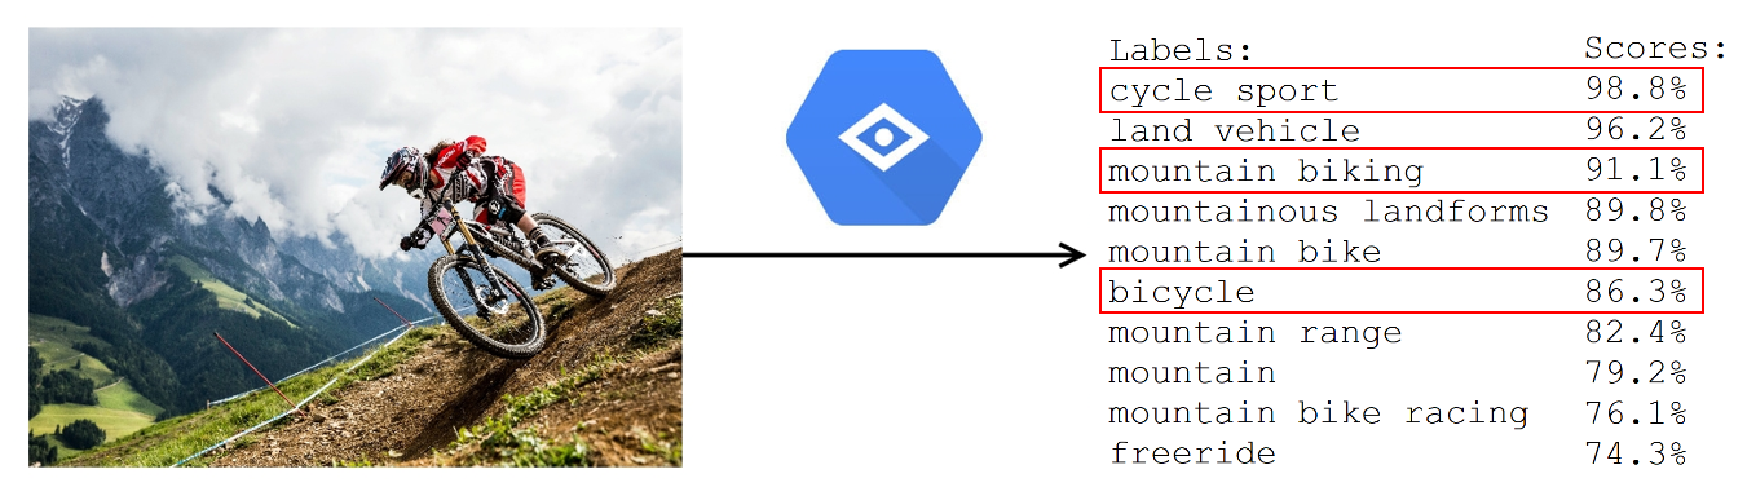
\includegraphics[width=0.75\textwidth]{img/vision_illustration}
\caption{This visualisation shall illustrate the image recognition process which is performed by the Google Cloud Vision API.}
\source{(1) Mountain biker - https://allaboutlimassol.com/assets/images/primary-image/ \\ 51024-0.downhill\_mountain\_biking.jpg, accessed: 30.03.2019 \\
(2) Vision emblem - https://cloud.google.com/vision/?hl=de, accessed: 30.03.2019}
\label{fig:vision_illustration}
\end{figure}

The placement of this entire step in relation to the other data- and text-processes is visualised in step 2 of figure \ref{fig:ml_visualisation}.

\subsection{Query costs} \label{vision_query_cost}
Google allows the creation of one Google Cloud trial account (needs a valid Credit Card for verification) per user which comes with 300 US Dollars' worth of credit. This credit can be used among others to rent virtual machines (VM's), access API's and other Google Cloud services.The Google Cloud Vision API can also be paid with that available credit and comes with the following rates: The first 1'000 requests per month are free of charge. Subsequent requests up to 5 million requests per month are charged at \$1.50 per 1'000 requests - this applies specifically to the API specific label detection feature. Therefore, the 300\$ worth of credit would allow the processing of around 201'000 images. These rates\footnote{https://cloud.google.com/vision/pricing, accessed: 29.03.2019} were in place during the time of writing (March 2019) and will mostly likely vary with time.

\clearpage

\section{Machine Learning for text classification} 

\subsection{Machine learning on non-numerical text data} \label{ml_text_data}

\begin{wrapfigure}{l}{0.3\textwidth} %0.3 and 0.28
  %\vspace{-0.5cm}
  %\begin{center}
    \centerline{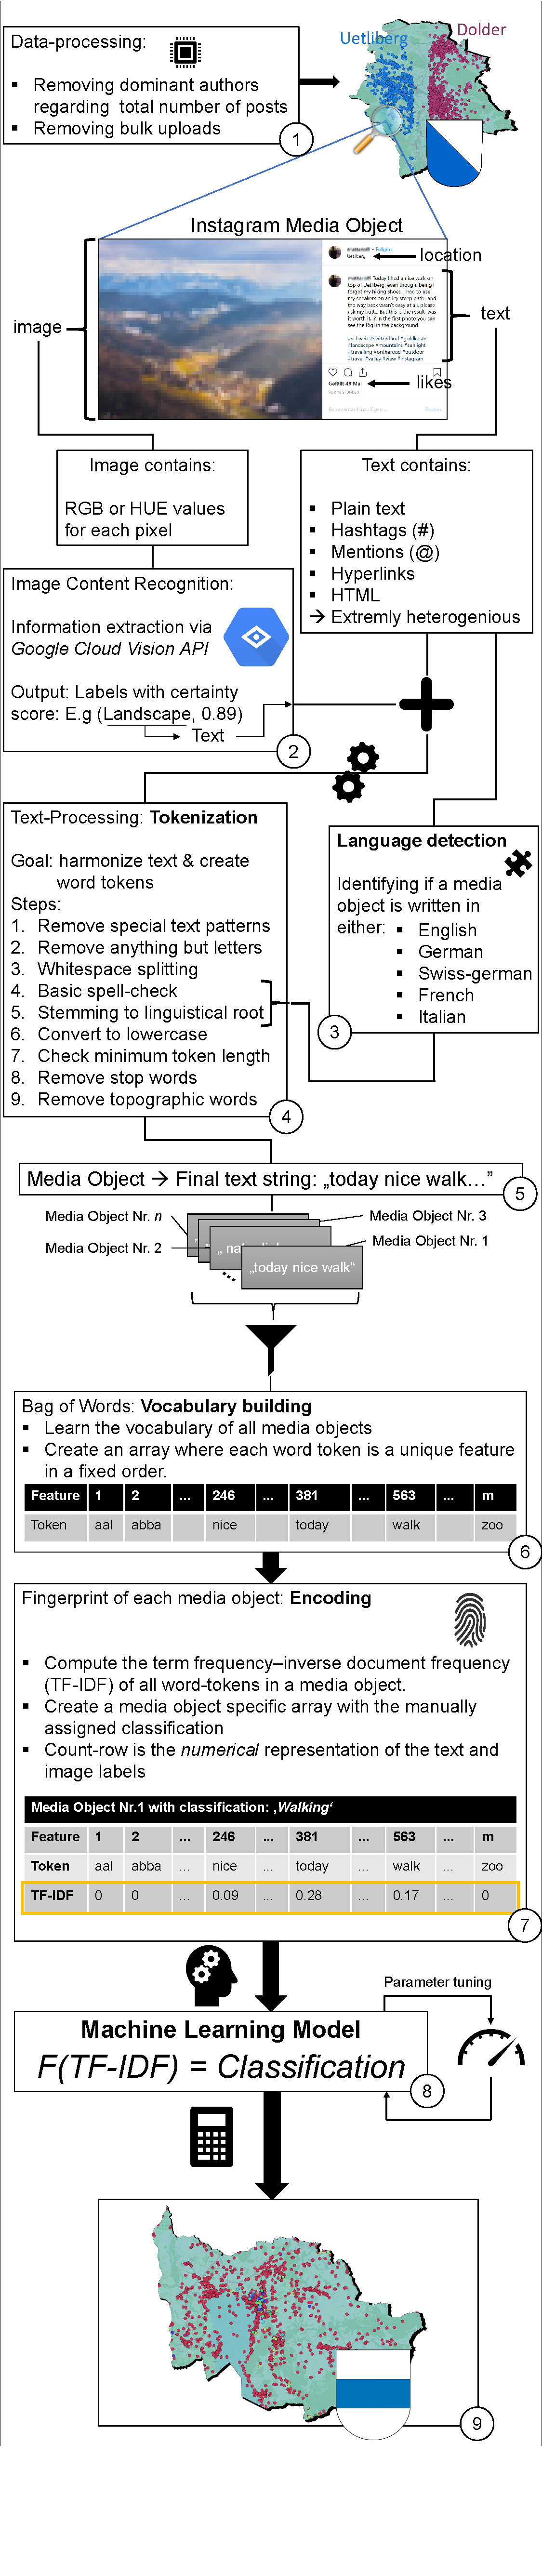
\includegraphics[trim={0 0 0 0},clip,width=0.28\textwidth]{img/ML_text_data_visualization_cropped.pdf}}
%if trimming and clip is necessary: \includegraphics[trim={5cm 0 0 0},clip]{example-image-a}
  %\end{center}
  \caption{Core ML workflow}
  \label{fig:ml_visualisation}
\end{wrapfigure}
One approach to transform text-based data into machine readable information will be covered in this section. Steps 3, 4, 5 and 6 of figure \ref{fig:ml_visualisation} to the left can be used as reference and will illustrate the described processes.\\
There are multiple approaches available to prepare text-data for a ML model but outputting numbers at the end in one form or the other is uniform.\\
In this project the \textit{bag-of-words} representation has been applied \parencite{Joulin2016}. This algorithm learns the 'vocabulary' of a corpus of documents or media objects in this case. The entire corpus-vocabulary is compared to the word-tokens incorporated in each media object. Therefrom, a fingerprint-like sequence of numbers is created which represents the occurrence and absence of words-tokens in the corresponding media object. The entire process can be boiled down to three steps\footnote{https://scikit-learn.org/stable/modules/feature\_extraction.html\#text-feature-extraction, accessed: 29.03.2019} which explain more thoroughly what has been said above:

\paragraph*{Tokenization} The input consisting of the concatenated text strings and the image recognition labels of each media object is processed into word- tokens by a sequence of various functions as seen in section \ref{text_processing} \textit{Text-processing} and step 4 of figure \ref{fig:ml_visualisation}. This homogenisation enables a reduced model complexity by merging similar features and neglecting features with little semantic meaning. The generated string outputs (see \ref{fig:ml_visualisation} step 5) are fed into:

\paragraph*{Vocabulary building} By assessing the individual word-tokens of each media object the \textit{bag-of-words} constructor assembles a vocabulary of unique tokens found in the corpus. This vocabulary comes in the shape of an alphabetic ordered array where each column represents a word token. These columns are from now on referred to as (model) features.

\paragraph*{Encoding} The previously build vocabulary array is iterated over and compared to the word tokens found in the final text-string of each media object for which a 'fingerprint'-array is instantiated. Missing words are recorded as nulls and appearances are recorded by their count. The final weight of each feature is calculated according to the \textbf{T}erm (feature) \textbf{F}requency inside the media object times the \textbf{I}nverse  \textbf{D}ocument  \textbf{F}requency (occurrence across all media objects) which is referred to as TF-IDF. This results in a number sequence linked to a given media object on which the model is later trained.

\clearpage

\subsection{Recreation-types} \label{recreation_types}
The decision which NBRAs the model should capture was built upon and influenced by the 'Recreation types Guidebook' of the Institute of Technology Rapperswil \parencite{IFL2018}. The following seven distinct classes were chosen for the model to be trained on:
\begin{enumerate}
    \item walking
    \item hiking
    \item jogging
    \item biking
    \item dog walking
    \item horse riding
    \item picnic
\end{enumerate}
The observation of similar appearing classes is true and one can argue about its effectiveness and the degree of overlapping. How would people differentiate between e.g. walking, hiking and jogging? The ground truthing as well as the SMD revealed (see results \ref{results}) that some people perceive a journey through a forest as hiking while for others it is still considered going for a walk. Normally, NBRAs can be easily identified and distinguished by the needed equipment. Not so much in the case of the three mentioned NBRAs compared to the other classes like horse riding where you notably need a horse.\\
Nevertheless, the classes 1-3 account for the majority of recorded NBRA-occurrences. 77\% of the entire manually verified training's data used to fit the model was classified as one of them. This clearly shows the importance of these NBRAs as well as their spatial distinction.
Additionally, a class 'None' is also implemented which describes a media object which is not related to nature recreation and therefore is not an entity of any of the above listed NBRAs.\\
\newline
If one is familiar with all the classes in the mentioned recreation types guidebook \parencite{IFL2018} than the absence of the NBRA 'Swimming/Bathing' would stand out. The reasoning behind the exclusion of said class is based on the Instagram data-acquisition period from the 30.09.2018 till the 11.12.2018. During this time little training's data was available on outdoor swimming due to the low lake temperatures. Additionally, the spatial occurrence of people swimming is less diverse and corresponds to certain well known locations. Considering these circumstances and the additional needed effort, the decision against the inclusion of 'swimming' as an independent class was made.

\subsection{Acquisition and preparation of the training- and test-dataset} \label{preparation_training_data}
Due to a limited amount of available Instagram and Flickr data of the research area and the entire Canton of Zug respectively it was certain that not enough training-data for each of the NBRA-types was available. Therefore, a larger additional Instagram dataset was drawn upon which was collected by the geocomputation team of the University of Zurich \parencite{Gruzd2016}. The dataset consisted of ten locations in Switzerland which differed in topography, spoken language and demographic factors. The locations were the following: Aarau, Arosa, Ebmatingen, Locarno Nord, Neuch\^{a}tel, Ovronnaz, Schanf, Scuol, Uetliberg and Zurich Dolder. For each location there existed around six to seven individual files that partly overlapped in the time they were acquired. The entire dataset covered a time-span of approximately three months for every of the mentioned locations from the beginning of October 2017 till the end of January 2018. A total of ten merge files - one for every location - were created to firstly eliminate any duplicate media objects and secondly to add the location name as an additional column to the data-rows for easier database filtering later on.\\
\newline
After considering the different topographic attributes ,the data-composition and quantity of all ten locations, Zurich Dolder and Uetliberg were chosen as sources for the training's data due to their similarity to the research area and to the overall Canton of Zug. This accounted for a total of 206'454 and 74'742 unique media objects respectively during pre data-processing. After neglecting the top seven authors in the case of Zurich Dolder and the top ten for the Uetliberg dataset (see: \ref{bias_dominant_authors}) as well as applying a common bulk upload threshold of five uploads per day (see: \ref{bias_bulk_uploads}), this led to a dataset reduction to 191'584 and 68'522 post data-processing respectively. Attentive readers will notice that the resulting ML model is purely based on Instagram data even though Flickr data is predicted with it as well. This observation is correct and can be legitimatised with the assumption that user generated text does not differ to heavily between SMPs. That this hypothesis hols true is shown in section \ref{precision_unseen_data}.\\
\newline
The next step encompassed the coarse identification of potential training's data for the seven given NBRAs. This was done with tailored SQL queries (see Appendix \ref{sql_queries_for_trainingdata}) to the \texttt{processed\_text}-column of the \texttt{media\_objects\_trainingdata\_instagram} database-table containing case insensitive regular expressions (see definitions) in the form of:

\[processed\_text \sim * (\backslash s | \wedge)KEYWORD(\backslash s | \$)\]

The following break-down of the query explains the parameters and search criteria in more detail. The SQL syntax \texttt{$\sim$*} initiates a case-insensitive regular expression matching with the database \texttt{processed\_text}-column of each media object. A regular expression (short: regex) is a sequence of characters used to describe and match a specific string pattern. The regex \texttt{($\backslash$ s | $\wedge$)} defines that the string-pattern of interest must either start with a whitespace ($\backslash$ s) or must be located at the beginning of the string ($\wedge$). Next follows the placeholder for potential keywords that are likely to occur in a media object of interest of a certain class. The used keywords must be run through the same text-processing algorithm - the way every media object in the database did - to allow for successful matching. Lastly, ($\backslash$ s | \$) defines that the string-pattern must either end on a whitespace or must be located at the end of the string.\\ 
Media objects that were selected through this process were labelled according to the matching NBRA by changing the classification column in the corresponding row in the database. The order in which these NBRAs were queried impacted the amount of entities a given class would acquire after the entire set was classified. This is given by the fact that certain media objects fit the criteria of multiple queries or NBRAs. Therefore, an already classified media object could be reclassified by a later query. The order in which the queries were eventually executed corresponds to the order in the table below (see table \ref{tab:trainingsdata}). The idea behind this approach was to reduce reclassification of media objects that belonged to an already weakly represented NBRA such as 'horse riding' or 'dog walking'. Simultaneously, this would help even out the number of training's data per classification which is sought-after for the ML training's process. It has to be noted at this point that any media object that was not targeted by any of the class specific SQL queries was automatically assumed to be of the None-class which resembles media objects that are unrelated to any of the mentioned NBRAs.\\
These 1'890 coarse pre-determined classifications were in a following step manually verified and changed if needed. This led to a deduction to a total of 1'046 remaining training's data objects (see \ref{tab:trainingsdata}). No media object with the pre-determined classification of 'None' was manually verified.\\
\newline
One issue that became apparent during the manual verification procedure was the problem of consistent class-definitions especially for classes that were closely related such as 'walking' and 'hiking'. As already touched upon before people tend to have different interpretations of what hiking and what walking is. Also hiking might sound more adventurous then walking which could explain an even more interchangeable usage in the field of social media. The following rules were established to differentiate between the three most similar classes: hiking, jogging and walking. A violation of these rules would lead to a reclassification during the manual verification process.

\begin{enumerate}
    \item Mentioned equipment: If equipment related keywords are present that give a strong incentive towards one class over another. E.g. 'backpack' for hiking.
    \item Mentioned adjectives, adverbs: It is assumed that these NBRAs can be allocated on an axis that goes from relaxing to adventurous. Walking being on the far left, followed by jogging in the middle and hiking on the far-right side. If adjectives or adverbs are used, that allow the allocation of a media object on this axis, then the closest most fitting class is chosen.
    \item Basic human context interpretation: If a media object is clearly incorrectly classified according to the (author of this thesis) human interpretation of the text then a reclassification is performed.
\end{enumerate}

The baseline being that the model is trained to capture the personal interpretation of the media object author of what he/she thinks the present NBRA is. Therefore, if no certain manual distinction between classes can be made then the used action verb decides the class. E.g.:\\
'We went for a walk on Uetliberg' $\to$ walking \\
'I went hiking on Uetliberg' $\to$ hiking\\

\begin{table}[ht]
\begin{center}
\caption{Training's data purification process}\vspace{1ex}
\label{tab:trainingsdata}
\begin{tabular}{llccc}\hline
NBRA & SQL query matches* & Classifications** & After manual verification \\ \hline
Walking & 549 & 485 & 333 \\
Hiking & 465 & 428 & 306 \\
Jogging & 377 & 358 & 208 \\
Picnic & 339 & 335 & 51 \\
Biking & 169 & 164 & 72 \\
Dog walking & 74 & 74 & 63 \\
Horse riding & 46 & 46 & 13 \\
None & - & 279'285 & 279'490 \\ \hline
\end{tabular}
\newline
*see Appendix **can get overwritten by other SQL queries
\end{center}
\end{table}

\subsection{Issue of expired Instagram media links} \label{expired_media_links}
Every media object acquired by the Instagram API or Netlytic contains a media link which points towards the embedded image, video itself. All these generated Instagram media links contain a time-stamp component which functions as an expiration date upon which the links become invalid \parencite{Wayne2018}. At the time of writing the training's dataset dates back more then one year and all the media links already turned invalid.\\
The links to the full Instagram media object (see section \ref{Instagram_data}) on the other hand were still valid - given the author of the media object or Instagram themselves did not take it down in the meantime. The media link of interest could be acquired by crawling through the web-page and finding the HTML \texttt{<div>} container which encompassed the correct \texttt{<img>} element with the id = "FFVAD". The source (\texttt{src}) attribute of that image element provided a valid media link that could be passed directly to the Google Cloud Vision API for the image recognition.

\subsection{Machine learning model} \label{ml_model}
The following subsections encompass the entire pipeline of functions that were used to build \textbf{two} kinds of models. These models should provide insight on the effect of combining text and image content data in regards to model performance. Therefore, the first model was solely trained on the processed user generated text-data whereas the second model was trained additionally on the processed image content labels that were returned from the Google Cloud Vision API. Aside from that the models were setup, trained, tuned and implemented in exactly the same fashion.\\
Scores for evaluating ML model performance are also introduced which are referenced again in the results. The entire code implementation of the subsequent steps can be found in Appendix \ref{python_code} and in digital form in the enclosed CD.

\subsubsection*{Considered algorithms} \label{ml_algorithms}
The following algorithms were tested and evaluated for the creation of the two ML models. The results will be presented in section \ref{results_models}.

\paragraph*{Support Vector Machines (SVMs)}
A SVM can be used for classification and regression applications. Its aim is to divide media objects of different classes - represented as vectors - by creating a hyperplane while maximising the distance between the closest vectors of each class (see hyperplane H\textsubscript{2} in figure \ref{fig:SVM_visualisation}). This constraint improves the performance of the model on new data where vectors do not follow the exact spatial distribution of the training's data.

\begin{wrapfigure}{l}{0.5\textwidth} %0.3 and 0.28
  %\vspace{-0.5cm}
  %\begin{center}
    \centerline{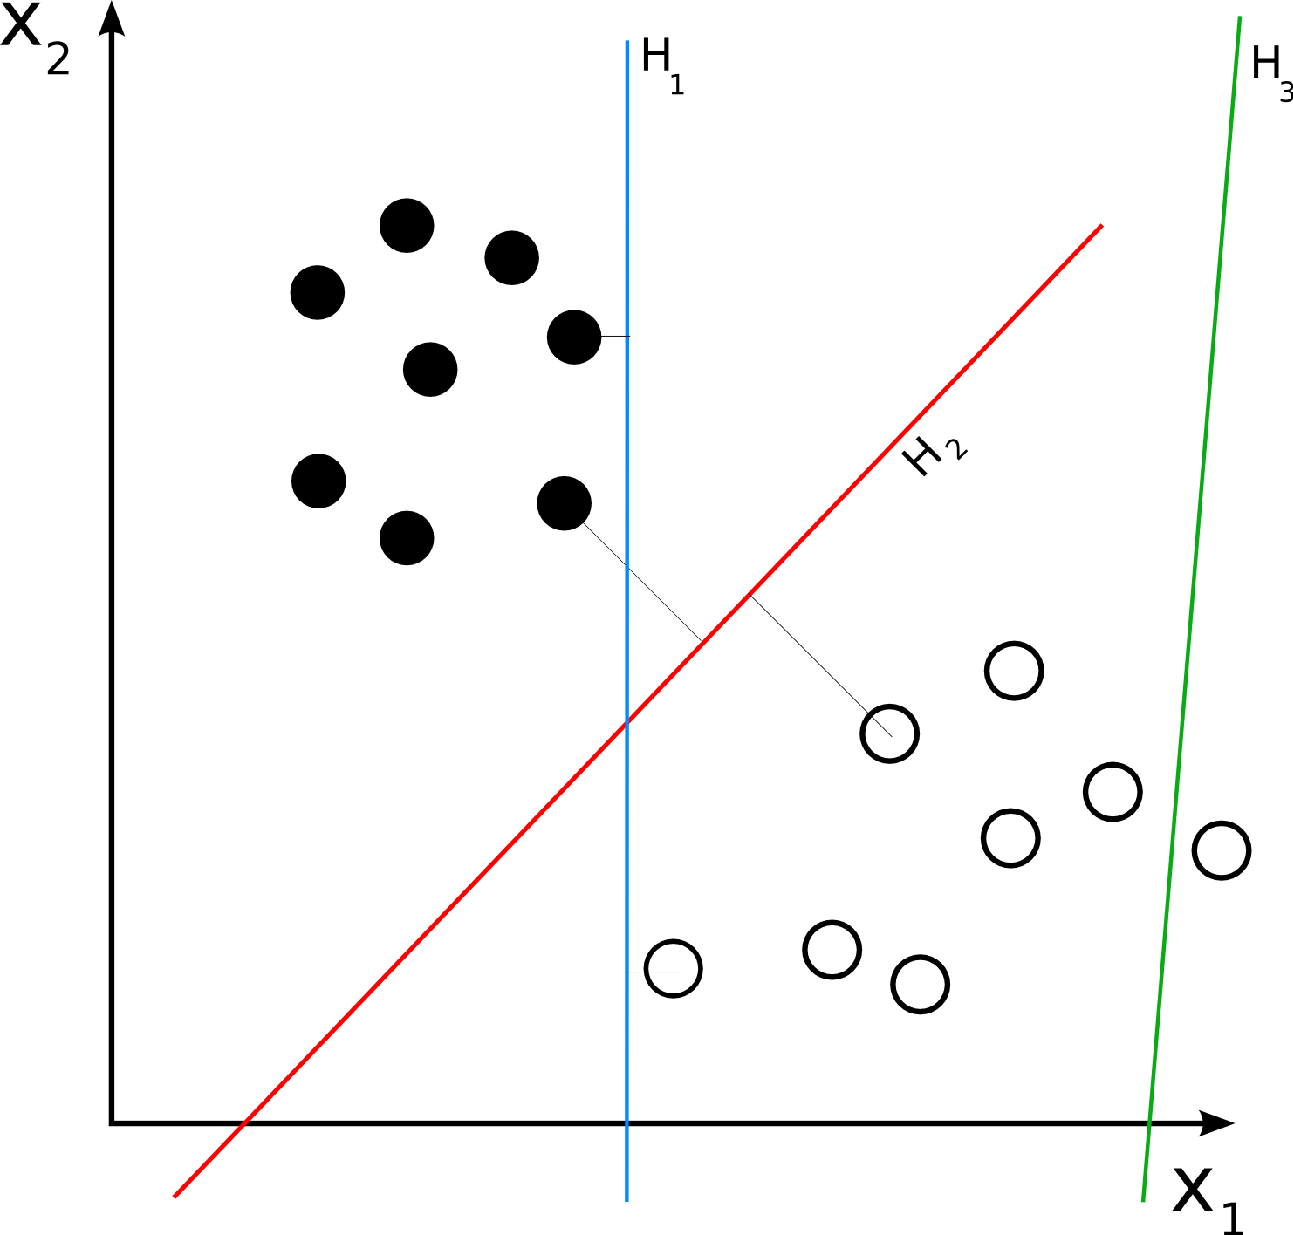
\includegraphics[trim={0 0 0 0},clip,width=0.28\textwidth]{img/Svm_separating_hyperplanes}}
%if trimming and clip is necessary: \includegraphics[trim={5cm 0 0 0},clip]{example-image-a}
  %\end{center}
  \caption{Visualisation of possible SVM fitted hyperplanes to separate two data-point clusters. H\textsubscript{3} does not manage to completely separate the clusters. H\textsubscript{1} does separate them entirely but violates the constraint to maximise the space between them, unlike H\textsubscript{2}.}
  \source{https://en.wikipedia.org/wiki/ \\ Linear\_classifier, accessed: 29.03.2019}
  \label{fig:SVM_visualisation}
\vspace{-0.5cm}
\end{wrapfigure}

For the calculation of the mentioned hyperplane are only the marginal vectors of relevance because they define the border between the classes and therefore the location of the plane. Name giving is the fact that only a small portion of the entire vector set - the so called support vectors - is used for the training of the model. The result is an algorithm with comparably low processing costs.

\paragraph*{Decision Tree algorithm}
Like SVMs decision trees can be used if a continuous value (regression) or a concrete set of values (classification) is desired as model output. Decision trees are fundamentally consecutive IF / ELSE statements (nodes) which try to purify the data with increasing tree depth. The determination of the nodes operation and their position inside the tree is seen as the fitting or training of the model.\\
One specific variation of the generic decision tree which has been tested for this project is the so-called randomForest. It creates a defined amount of individual decision trees which are trained on different random test- and train-splits of the training's dataset. This process comes close to performing a cross-validation. At the end these trees are logically merged where deterministic features are kept and ones that carry little information are dropped. The result is a decision tree which more successfully captures the information contained in the training's data while reducing the trend to overfitting.\\
Decision trees are prone to overfitting due to their infinite possible depth by adapting perfectly to any training's dataset. This can be countered by limiting the maximal depth of the tree(s) (see listing \ref{coderandomForestparameters}) . This process is called pre-pruning.\\
\newline
 The book from \textcite{Guido2016} about ML stated that "random forests do not tend to perform well on very high dimensional, sparse data, such as text data". Nevertheless, this algorithm was tested and did not perform much worse than the linearSVC model (see section \ref{results_models}. Due to the fact that the calculation process of the different decision trees can be multithreaded across all available CPU cores, the fitting process can be faster than the one of the linearSVC model (in this thesis roughly 15\% faster). 

\subsection{Model setup} \label{model_setup}
In addition to the previously mentioned data- and text-processing steps some extra functions were needed before the actual fitting algorithm could be applied. The models were setup with Python v.3.6.7 and the \textit{scikit-learn} library v.0.20.2. This library allowed pipelining\footnote{https://scikit-learn.org/stable/modules/compose.html, accessed: 29.03.2019} (see definitions) which consisted of the following functions:

\begin{enumerate}
    \item \textbf{TfidfVectorizer} Converts a collection of raw documents (media objects) into a matrix of TF-IDF features which stands for the frequency times the inverse document frequency of a given word-token (see step 5 and 6 of figure \ref{fig:ml_visualisation}). This function is equivalent to applying 'CountVectorizer' followed by 'TfidfTransformer'.\\
    \textit{Tuned hyper-parameters:}
    \begin{itemize}[label={}]
        \item \textbf{Min\_df} This parameter defines the minimal required document frequency of a word-token in the entire corpus to be included for further processing.
        \item \textbf{Ngram\_range} This parameter defines how word-tokens are interpreted by the model. Given a minimal and a maximal value the function is able to create new features by concatenating tokens that appear in succession. This enables the extraction of semantic meaning that would stay unseen if only individual token were considered \parencite{Surtikanti2013}. E.g (1,2) would consider all single tokens as well as the concatenation of two consecutive tokens. (2,3) would only consider token concatenations of length two up to a maximum of three.
    \end{itemize}
    
    \item \textbf{SelectKBest} This function allows for a further selection of the features generated by the vectorizer. Score functions such as ANOVA F-value and Chi-squared allow the selection of the most deterministic features in a set. Limiting the number of features can help to prevent model overfitting and increase a model's generalisation capabilities.\\
    \textit{Tuned hyper-parameters:}
    \begin{itemize}[label={}]
        \item \textbf{k} Defines the number of further considered features with the highest score.
    \end{itemize}
    
    \item \textbf{ML algorithm} LinearSVC and randomForest classifiers (see section \ref{ml_algorithms}) were used to find the most well-rounded model.\\
    \textit{Tuned hyper-parameters:}
    \begin{itemize}[label={}]
        \item \textbf{LinearSVC \textit{C}} Adjusting this parameter gives the user control over the margin-size of the hyperplane. This effects how strong the model is fit to every single training's point. Reducing this parameter allows for more generalisation and counteracts to overfitting. Increasing the 'C' parameter raise the model's training's accuracy (see figure \ref{fig:over_underfitting}).
        
        \item \textbf{LinearSVC Penalty} This parameter introduces a regularisation penalty to prevent overfitting by minimising the components of the word-token vectors. There are two commonly used L\textsubscript{p}-norms:
        \begin{itemize}[label={}]
            \item \textbf{L1} Favours sparse parameter vectors which helps to identify important features.
            \item \textbf{L2} Forces parameter vectors to be close to zero.
            \item For more detailed information on these two regularisation terms with an in depth comparison please refer to \textcite{Mazilu2011}.
        \end{itemize}
        
        \item \textbf{randomForest n\_estimators} Defines the amount of independent decision trees that are created. The higher the number the better are classification boundaries smoothed and the training's data captured. The downside is the computational cost increase.
        
        \item \textbf{randomForest max\_depth} Defines the number of levels the created decision trees are made of.
    \end{itemize}
    
    \item \textbf{GridSearchCV} This function allows the systematic testing of different hyperparameter settings to find the best performing configuration. This process is also known as model tuning. The weighted F1-score instead of the default accuracy score was used to evaluate performance of the individual models due to the multi-classification approach. Additionally, cross-validation is performed to ensure the result reliability (leave one out cross-validation has not been considered due to the great increase in processing time). The used hyperparameter testing grid for the randomForest algorithm is visible in figure \ref{coderandomForestparameters} and the one for the linearSVC algorithm in figure \ref{codelinearsvcparameters}.
\end{enumerate}

\begin{lstlisting}[language=Python, caption=Tuned hyperparameters of the randomForest fitting algorithm, label=coderandomForestparameters]
randomforest_parameters = {
                    'vect__min_df': [9, 10, 11, 12, 13, 14],
                    'vect__ngram_range': [(1, 1), (1, 2), (2, 2), (1, 3)],
                    'chi__k': [500, 600, 700, 'all'],
                    'clf__max_depth': [5, 6, 7, 8, 9, 10, 11, 12, 13, None]
                }
\end{lstlisting}

\begin{lstlisting}[language=Python, caption=Tuned hyperparameters of the linearSVC fitting algorithm, label=codelinearsvcparameters]
linear_svc_parameters = {
                    'vect__min_df': [7, 8, 9, 10, 11, 12, 13],
                    'vect__ngram_range': [(1, 1), (1, 2), (2, 2), (1, 3)],
                    'chi__k': [500, 600, 700, 'all'],
                    'clf__C': [0.001, 0.1, 1, 10, 100]
                }
\end{lstlisting}

\texttt{Remark:} At the end the model was trained on the entire training dataset with the best parameter configuration.\\

\subsection{Evaluation scores} \label{ml_evaluation_scores}
There are different measurements to evaluate a ML model. All of them can be extracted from the confusion matrix created during the testing phase of the model. This matrix consists of rows that represent the actual classes and columns that represent the class predictions. The name confusion matrix stems from the purpose of noticing if the model is confusing classes.

\begin{wrapfigure}{LR}{0.5\textwidth} %0.3 and 0.28
  %\vspace{-0.5cm}
  %\begin{center}
 % \renewcommand{\thempfootnote}{\arabic{mpfootnote}}
    \centerline{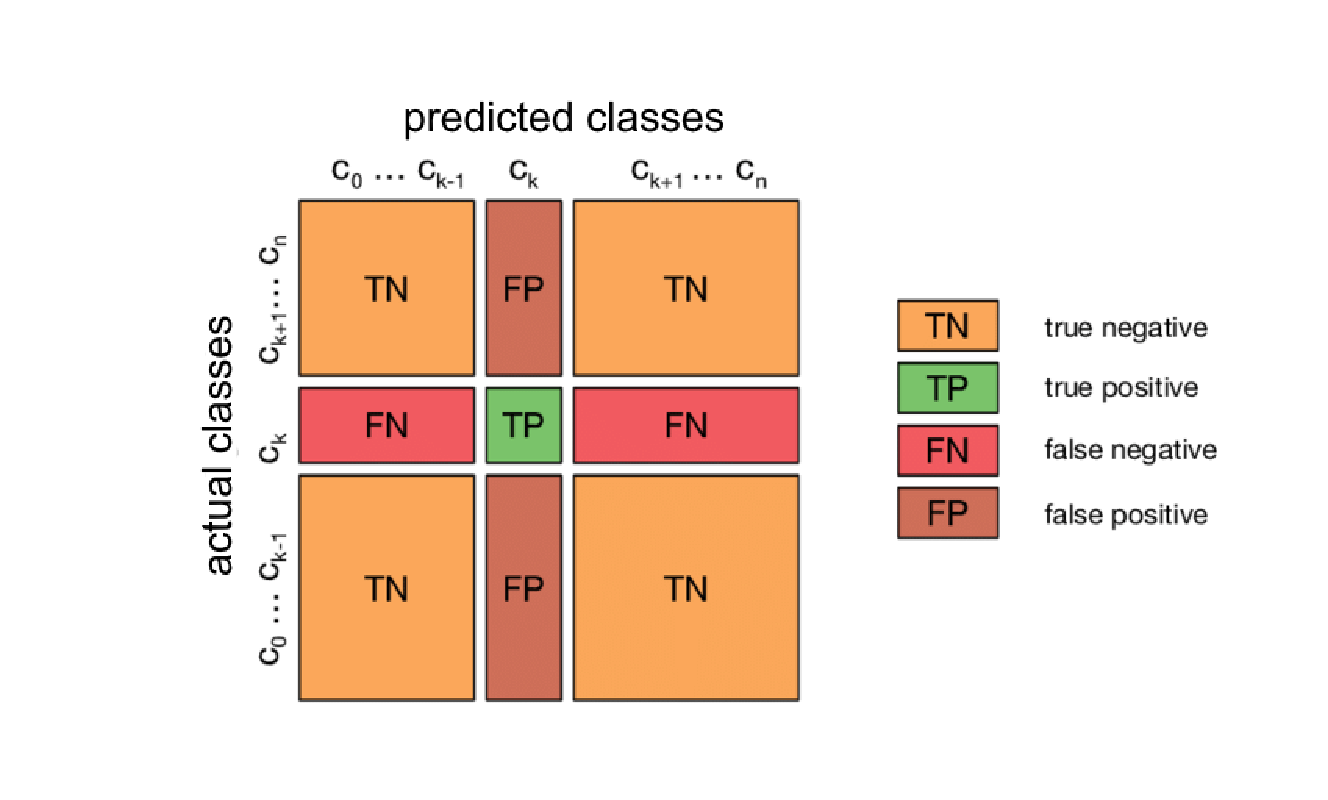
\includegraphics[trim={0 0 0 0},clip,width=0.49\textwidth]{img/Confusion_matrix_edited}}
%if trimming and clip is necessary: \includegraphics[trim={5cm 0 0 0},clip]{example-image-a}
  %\end{center}
  \caption{Confusion matrix with \textit{n} classes. When considering the class k (0 $\le$ k $\le$ n), the four different classification results can be obtained: true positive (green), true negative (orange), false positive (brown), and false negative (red).}
  \source{https://www.researchgate.net/figure/Confusion-matrix-for-multi-class-classification-The-confusion-matrix-of-a\_fig7\_314116591, author: Frank Kr\"uger, accessed: 29.03.2019}
  \label{fig:confusion_matrix_illustration}
\end{wrapfigure}

Measurements that were calculated (Abbreviations explained in the legend of figure \ref{fig:confusion_matrix_illustration}):

\begin{gather*}
accuracy = \frac{(TP+TN)}{(TP+TN+FP+FN)}\\
precision = \frac{TP}{(TP+FP)}\\
recall = \frac{TP}{(TP+FN)}\\
F1 = 2*\frac{(precision*recall)}{(precision+recall)}
\end{gather*}

\textit{F1-Score: Summarising Precision and Recall in one measurement.}

\clearpage

\section{Ground truthing} \label{groud_truthing}
Interviews and passive observations were performed to gain insight on how well the social media data approximates to actual visitation rates and spatial NBRA dispersion. This ground truth information shall help to answer the question on how good of a proxy the considered social media platforms and their data in the study area are.

\subsection{Locations for ground truth data acquisition} \label{locations_ground_truthing_data}

\begin{wrapfigure}{LR}{0.4\textwidth} %0.3 and 0.28
  %\vspace{-0.5cm}
  %\begin{center}
    \centerline{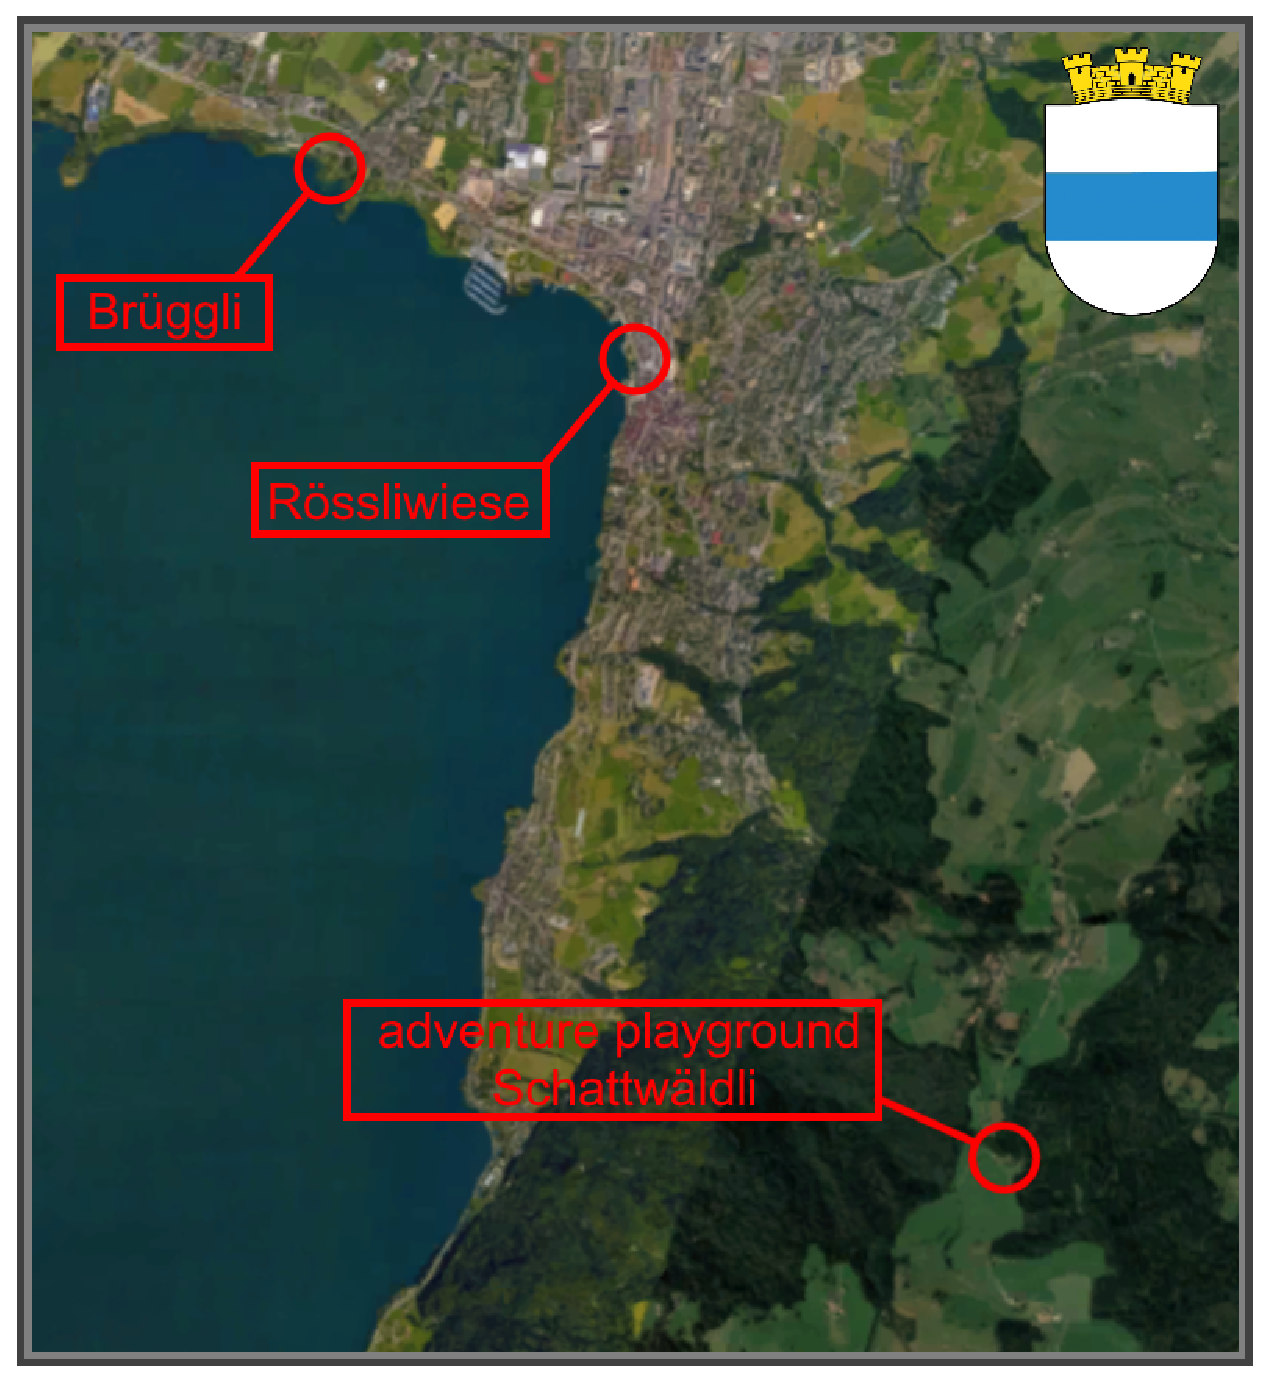
\includegraphics[trim={0 0 0 0},clip,width=0.39\textwidth]{img/interviews_locations}}
%if trimming and clip is necessary: \includegraphics[trim={5cm 0 0 0},clip]{example-image-a}
  %\end{center}
  \caption{Map visualising the locations where ground truthing in the form of interviews and passive NBRA observations were performed.}
  \source{\copyright Google, map-data 2019}
  \label{fig:locations_ground_truthing}
%\vspace{-0.5cm}
\end{wrapfigure}

Three locations (see figure \ref{fig:locations_ground_truthing}) with different degrees of urbanisation were chosen which resemble hotspots for NBRAs covered in this thesis. The location to the far left is called 'Br\"uggli' - right next to a camping ground - which resembles a hotspot for jogging, biking, (dog-) walking and in summer also for picnicking and swimming. It lies inside the perimeter of the concept 'Lorzenebene' (plain of the river Lorze) and is close to the 'Delta' wildlife sanctuary which allows for various activities along the lake for relaxation.\\
The second location includes the 'R\"ossliwiese' which is a meadow located close to the city centre at the lake side. There people like to go for short walks (with their dog), eat lunch, relax (after shopping). Its high attractiveness is mostly given by the closeness to the residential area.\\
The last and most nature-near location was the adventure playground 'Schattenw\"aldli' on the Zugerberg. It appeals to various groups of people due to its wide spectrum of activities the environment allows. Young families with kids are the most dominant visitor group due to the playground and the possibility to have a picnic. But also people hiking, walking (their dog) and mountain-bikers can be frequently encountered there.

\subsection{Passive observation setup} \label{passive_observation_setup}
The passive observation encompassed the recording of NBRAs performed by people that passed through the location during the same time the interviews were held. More specific the group size, the approximate average group age, the NBRA and the time were captured. The term 'passive' implies that no direct interaction with the recorded people occurred. Therefore, the data is entirely based on perception.
Since the thesis's author held all the interviews, the passive observation was performed by an unaffiliated assistant (see \nameref{acknowledgements}).\\
The durations of these passive observations were the following:
\begin{itemize}
    \item \textbf{Br\"uggli} 1h30min
    \item \textbf{R\"ossliwiese} 1h15min
    \item \textbf{Schattenw\"aldli} 1h45min
\end{itemize}
The time spend in one location was dependant on the time needed to hold the required interviews therefore the observable differences. Also, the relation between the observed frequencies of NBRAs were of greater interest than the actual recorded numbers.
The passive observation template used in this thesis can be found under Appendix \ref{passive_obs_templates}.

\subsection{Interview setup} \label{interview_setup}
A total of \textbf{52} interviews were performed in the afternoon during slightly cloudy but sunny conditions on the 24\textsuperscript{th} in 'Br\"uggli' (18 interviews) and 'R\"ossliwiese' (17 interviews) as well as on the 25\textsuperscript{th} of November 2018 in 'Schattenw\"aldli' (17 interviews). It was tried - to the best abilities of the author - to interview homogeneously across different age groups and NBRAs.\\
Every interview started out with a small introduction to the author's persona and the motivation behind the interviews. Additionally, the interviewees were informed that all the gathered information will be kept anonymous and used only within the scope of this thesis. The purpose of these interviews was to gain information on three topics.\\
\newline
The first one being \textbf{location} related:
\begin{itemize}[label={}]
    \item \textbf{Reason} Why was the current location in particular sought out? What was the motivation that resulted in visiting this location over another?
    \item \textbf{Activity} Which NBRA is currently practised by the person in this location?
    \item \textbf{Frequency} How often does the person visit the location? (In the case of 'Schattenw\"aldli', it was also asked what the destination of the trip was.)
\end{itemize}

The second one was related to \textbf{social media}:
\begin{itemize}[label={}]
    \item \textbf{Member} Do they own an account on any social media platform and if yes on which?
    \item \textbf{Habits} How do they interact with social media? Do they share own content (if yes in what frequency?), or do they rather look at contributions of others?
    \item \textbf{Intent} Do they consider sharing their current visit to the given location on social media and if yes on which platform?
\end{itemize}
The final topic at the end of the interview was dedicated to some person specific details. This included their age, gender, place of residence as well as the travel time to the location and their choice of transportation.\\
The interview template used in this thesis can be found under Appendix \ref{interview_templates}.
















